\selectlanguage{italian}%

\section{Soluzione}


\subsection{Schematici}

\begin{figure}[H]
	\centering
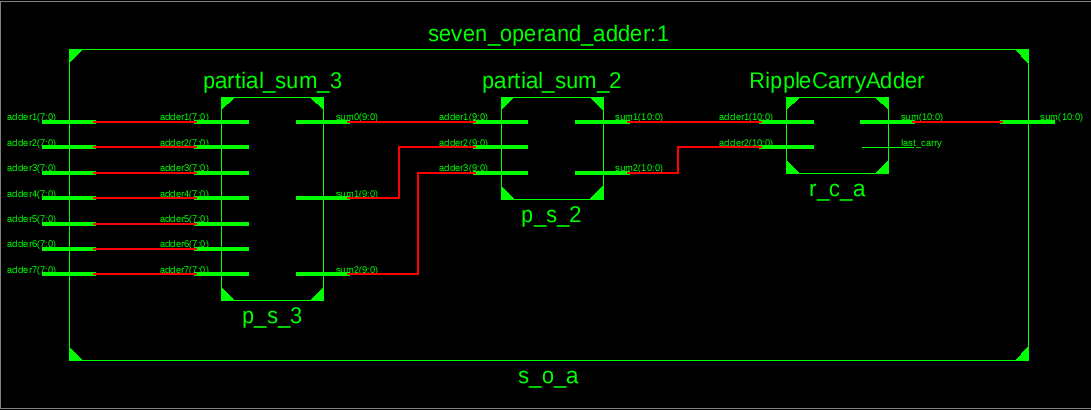
\includegraphics[scale=0.45]{esercizio12/images/seven_operation_adder.png}
	\caption{Seven Operand Adder}
\end{figure}

L' addizionatore � costituito dapprima da un dispositivo che trasforma
i sette input in ingresso in soli tre input da nove bit ognugno, grazie
al componente seven to three il quale conta il numero di uno presenti
in ingresso, di questi ne sono presenti otto ed ognugno ha in ingresso
bit dello stesso peso appartenenti a ciascuno operando, i valori in
uscita di tali componenti prima di essere passati al successivo vengono
incolonnati introducendo degli zero fittizzi per fa s� che le tre
stringhe di bit in uscita abbiano lo stesso peso(se pensiamo al primo
seven to three genera un bit di peso zero, uno di peso uno e l' ultimo
di peso due, questi vanno associati a tre strighe diverse ma le stringhe
con il bit di peso uno e due hanno bisogno di zero antecedenti per
poter incollonare le somme). Il partial sum due non sono altro che
dei full adder utilizzati come carry save, per produrre due stringhe
che vengono fatte sommare da dei Ripple Carry Adder, facendo le stesse
considerazione sui pesi discusse nel passo precedente.

\subsection{Codice}

\href{run:progetti/carry_select_adder/carry_seven_adder.xise}{Seven Adder ISE}

\selectlanguage{italian}%

